\subsection{¿Qué hacer si se muestra un error de STEAM al iniciar \textit{Alliance}?}

Si al iniciar \textit{Alliance} nos encontramos con un error como el de la figura \ref{ErrorSteam}, tan sólo tendremos que iniciar sesión en una cuenta de STEAM y reiniciar \textit{Alliance}. El error se debe a que el juego para su funcionamiento online usa el subsistema online de STEAM y sin iniciar sesión en STEAM no se puede hacer uso del mismo.

\begin{figure}[h]
  \centering
  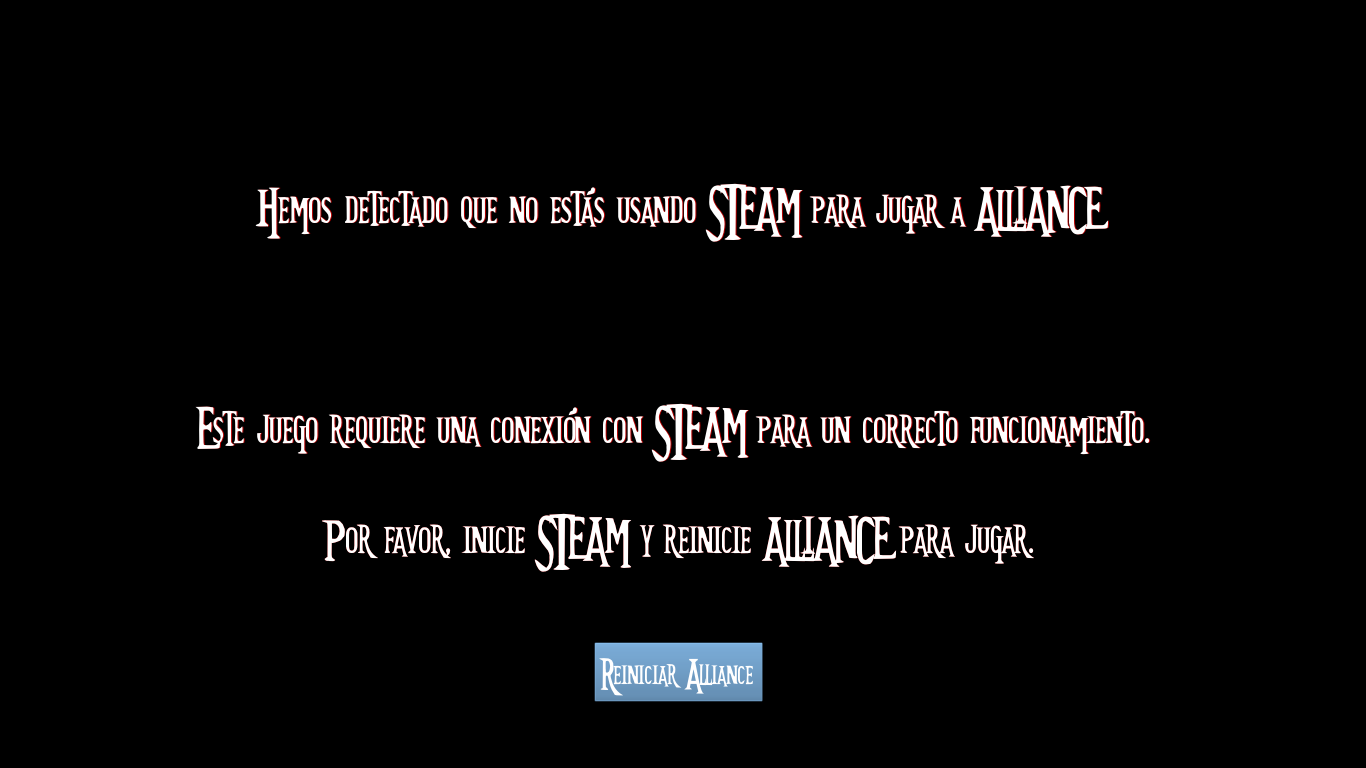
\includegraphics[width=12cm]{./images/ErrorSteam.png}
  \caption{Error de STEAM al iniciar el juego}
  \label{ErrorSteam}
\end{figure}


\subsection{¿Cómo jugar una partida de \textit{Alliance}?}

\begin{itemize}
\item En primer lugar, haz click en el ejecutable de \textit{Alliance}, para iniciar la aplicación.
\item Aparecerá el menú principal del juego, que se puede ver en la figura \ref{MenuPpal}.

\begin{figure}[h]
  \begin{minipage}{0.5\textwidth}
    \centering
    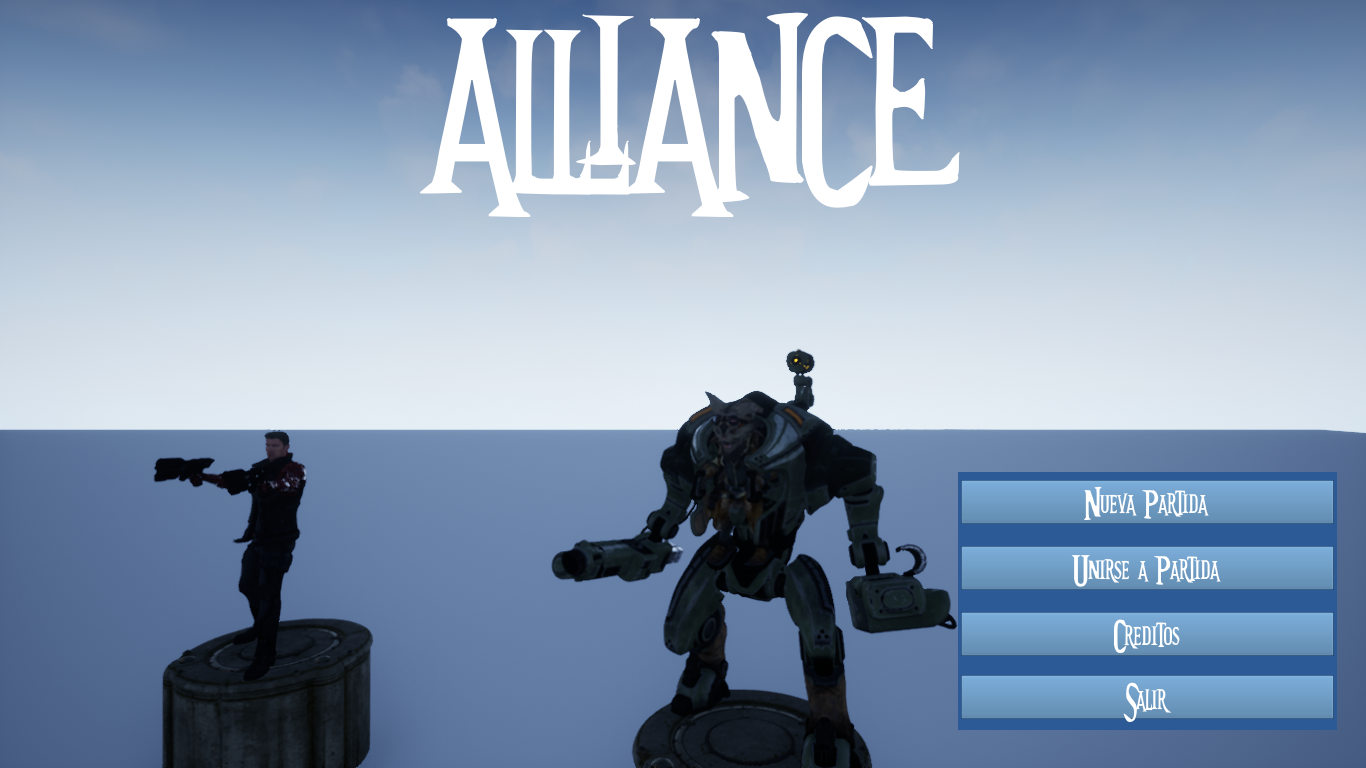
\includegraphics[width=8cm]{./images/MenuPpal.png}
    \caption{Menú principal de \textit{Alliance}}
    \label{MenuPpal}
  \end{minipage}%
  \hspace{1mm}
  \begin{minipage}{0.5\textwidth}
    \centering
    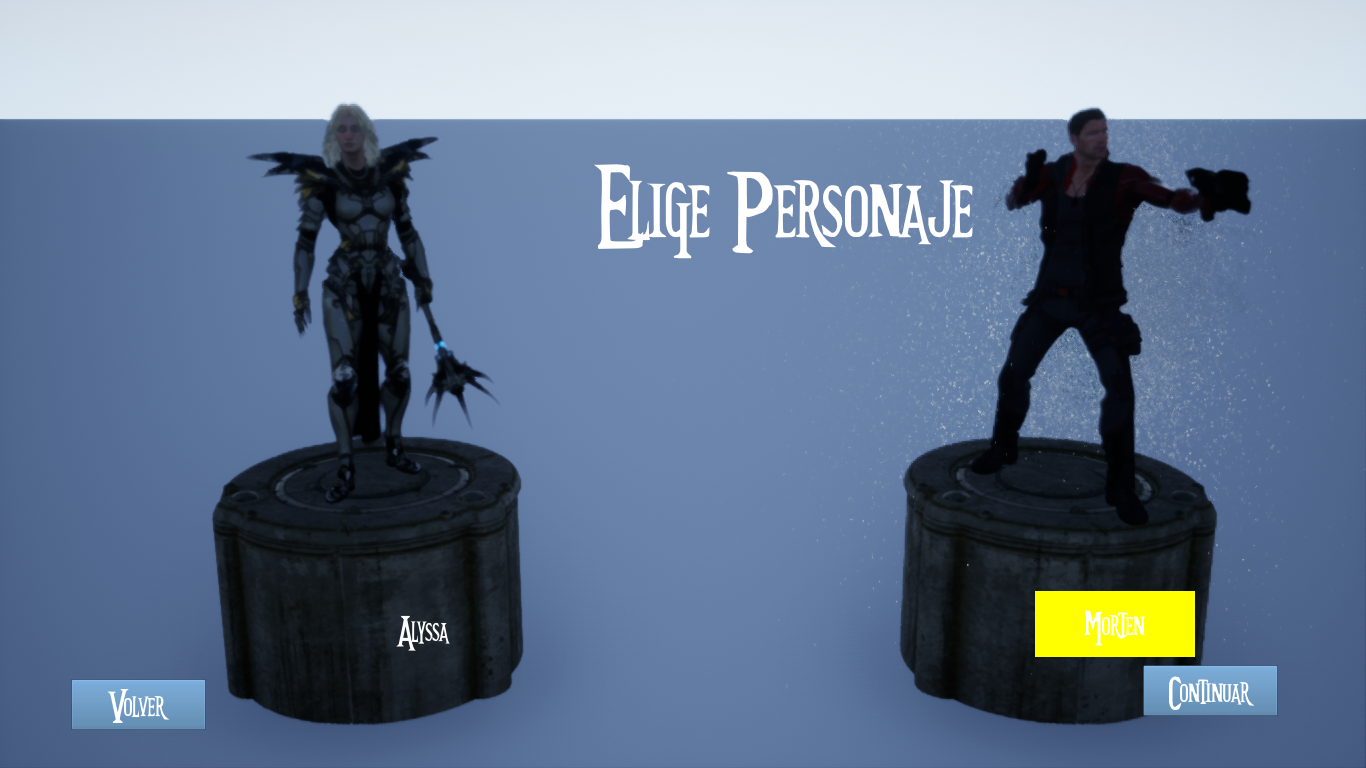
\includegraphics[width=8cm]{./images/EleccPers.png}
    \caption{Elección de personaje}
    \label{EleccPers}
  \end{minipage}
\end{figure}

\item En este menú haremos click en <<Nueva Partida>> para iniciar una nueva partida, la cual vamos a <<\textit{hostear}>>. Esto quiere decir que actuaremos como servidor en el caso de que se una un segundo jugador a nuestra partida. 

\item En la interfaz de la figura \ref{EleccPers}, se puede observar un \textit{zoom} sobre los personajes principales. Elegimos al personaje con el que queramos jugar, haciendo click en el botón con su nombre. Podemos reconocer nuestra selección gracias a las partículas existentes detrás del personaje elegido. 

\item Una vez estemos seguros de la elección de personaje, hacer click en <<Continuar>>. Saldrá una pantalla de carga tras la cual apareceremos en el inicio del primer nivel, y podremos jugarlo.
\end{itemize}


\subsection{¿Cómo unirme a una partida de \textit{Alliance}?}

\begin{itemize}
\item En primer lugar, haz click en el ejecutable de \textit{Alliance}, para iniciar la aplicación.
\item Aparecerá el menú principal del juego, que se puede ver en la figura \ref{MenuPpal}.
\item En este menú haremos click en <<Unirse a Partida>> para unirnos a una partida ya existente.

\begin{figure}[h]
  \begin{minipage}{0.5\textwidth}
    \centering
    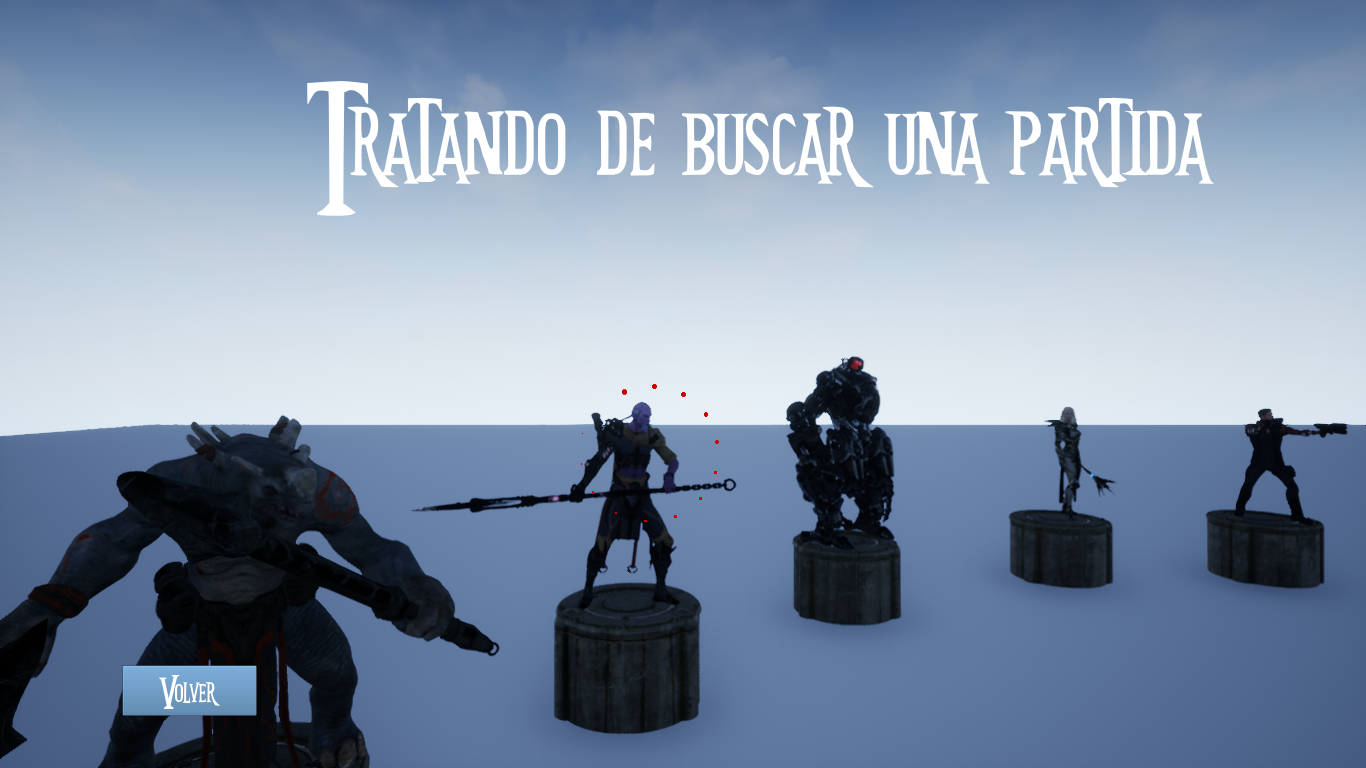
\includegraphics[width=8cm]{./images/BuscandoPartida.png}
    \caption{Buscando partida...}
    \label{BuscandoPartida}
  \end{minipage}%
  \hspace{1mm}
  \begin{minipage}{0.5\textwidth}
    \centering
    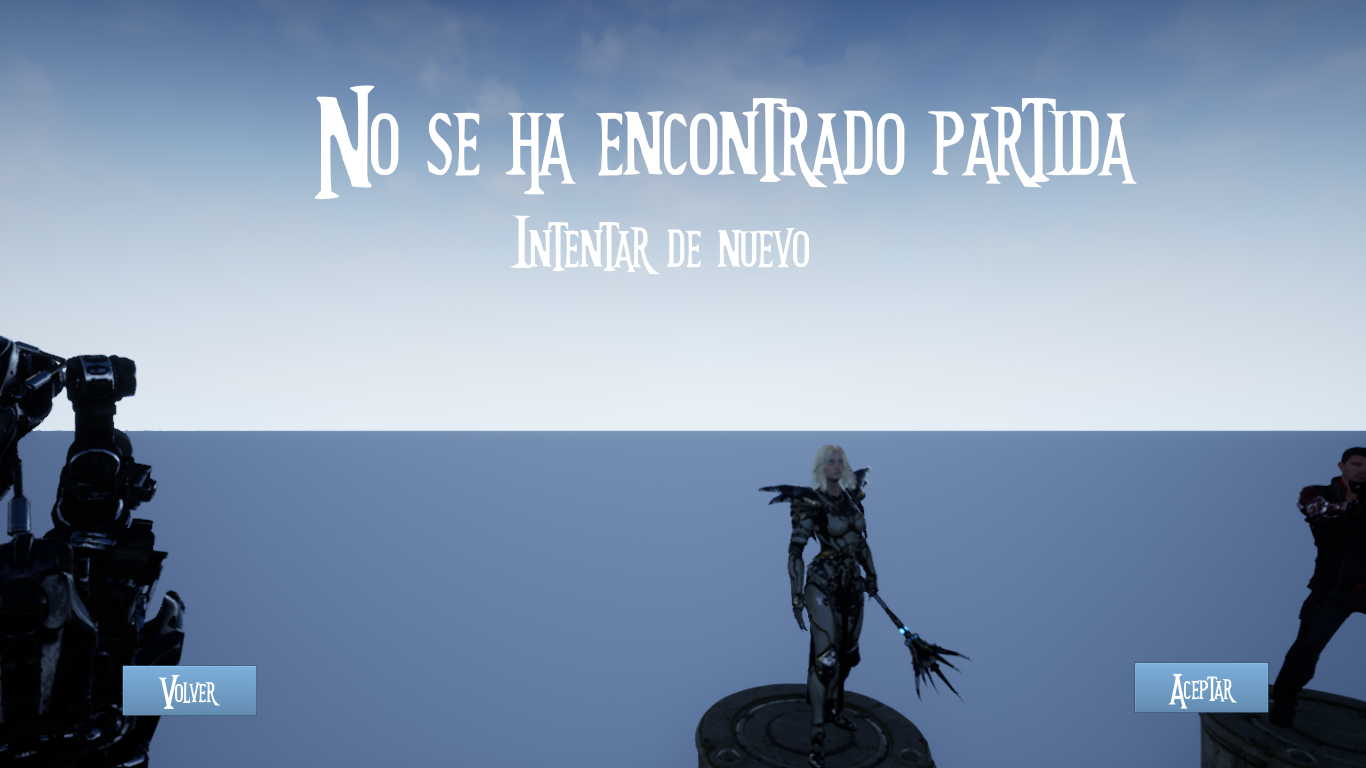
\includegraphics[width=8cm]{./images/PartidaNoEncontrada.png}
    \caption{Error. Partida no encontrada}
    \label{PartidaNoEncontrada}
  \end{minipage}
\end{figure}

\item Inmediatamente \textit{Alliance} comenzará a buscar una partida a la cual puedas unirte, como puede observarse en la figura \ref{BuscandoPartida}. En el caso de que no haya partidas a las cuales puedas unirte, saldrá el mensaje de error que se muestra en la figura \ref{PartidaNoEncontrada}. Puedes realizar una nueva búsqueda haciendo click sobre <<Aceptar>>.

\item Si se encuentra una partida a la cual puedas unirte aparecerá, una pantalla como la de la figura \todo{Insertar figura de éxito al unirse a partida}. Saldrá una cuenta atrás de diez segundos para que aceptes unirte a la partida. Si pasados los diez segundos no te has unido a la partida, deberás proceder a realizar una nueva búsqueda de partidas.

\item Una vez que se ha aceptado unirse a una partida, saldrá una pantalla de carga y tras esta, apareceremos en el nivel en el que se encuentre el jugador que \textit{hostea} la partida, controlando al segundo personaje principal no controlado por el \textit{host} de la partida.
\end{itemize}


\subsection{¿Cómo salir del juego?}

Existen varias maneras de salir del juego, dependiendo de si te encuentras jugando alguno de los niveles de \textit{Alliance}, o si te encuentras navegando por el menú principal (véase Figura \ref{MenuPpal}).

\begin{itemize}
\item \textbf{Si te encuentras navegando por el menú principal.}

Volver hacia las opciones del principio (haciendo click en <<Volver>>), que se muestran en la Figura \ref{MenuPpal}. Una vez en dichas opciones, hacer click en <<Salir>>.

\item \textbf{Si te encuentras jugando alguno de los niveles.}

\begin{itemize}
\item Pausar el juego, presionando la tecla \texttt{P} (o la tecla Escape) y hacer click en <<Salir del juego>>.
\item Dejar que los enemigos nos maten. En la interfaz que aparece (véase Figura \todo{Insertar imagen cuando el jugador pierde}), hacer click en <<Volver al Menú>>. Una vez en el menú principal, escoger la opción <<Salir>>, como se ha indicado anteriormente. 
\end{itemize}
\end{itemize}

\renewcommand\bcStyleTitre[1]{\large\hspace*{1.8in}\textcolor{red!100}{#1}}
\begin{bclogo}[
  couleur=red!15,
  arrondi=0.25,
  logo=\hspace*{1in}\bctakecare,
  barre=none,
  noborder=true]{\hspace*{0.15in} Advertencia.}
\itshape \vspace*{0.15in}
\textit{Alliance} no implementa un sistema de guardado de partidas, por lo que si sales de una partida, no se guardará tu progreso. La próxima vez que inicies \textit{Alliance} deberás empezar una partida nueva, comenzando el juego desde el principio.
\end{bclogo}


\subsection{¿Cómo jugar el minijuego?}

El minijuego que se ha implementado en \textit{Alliance} como mecanismo para abrir ciertas puertas es el clásico <<Klotski>>. Este juego se compone de un tablero, sobre el cual se colocan varias fichas de distintos tamaños y en distintas orientaciones. Existe una ficha, de color rojo (generalmente), que es la que necesitamos mover hacia la salida para ganar. Los únicos movimientos permitidos son horizontales y verticales sobre cada ficha, siempre y cuando haya espacio que lo permita.

En la implementación virtual, existen fichas de colores azules y rojo. La ficha con color rojo es la ficha que hay que llevar al hueco verde para conseguir ganar el minijuego y abrir la puerta. 

Tan sólo se puede mover una ficha si se ha seleccionado. Sabemos si una ficha está seleccionada porque su color cambia a rosa, como se puede ver en la Figura \ref{Minijuego}, y la selección de fichas se realiza pulsando la combinación de teclas \texttt{SHIFT+E} (para seleccionar la siguiente pieza) y \texttt{SHIFT+Q} (para seleccionar la pieza anterior).

Para mover una ficha seleccionada, se usan las teclas \texttt{W} (para mover la ficha hacia arriba), \texttt{S} (para moverla hacia abajo), \texttt{A} (para moverla hacia la izquierda) y \texttt{D} (para moverla hacia la derecha).

\begin{figure}[H]
  \centering
  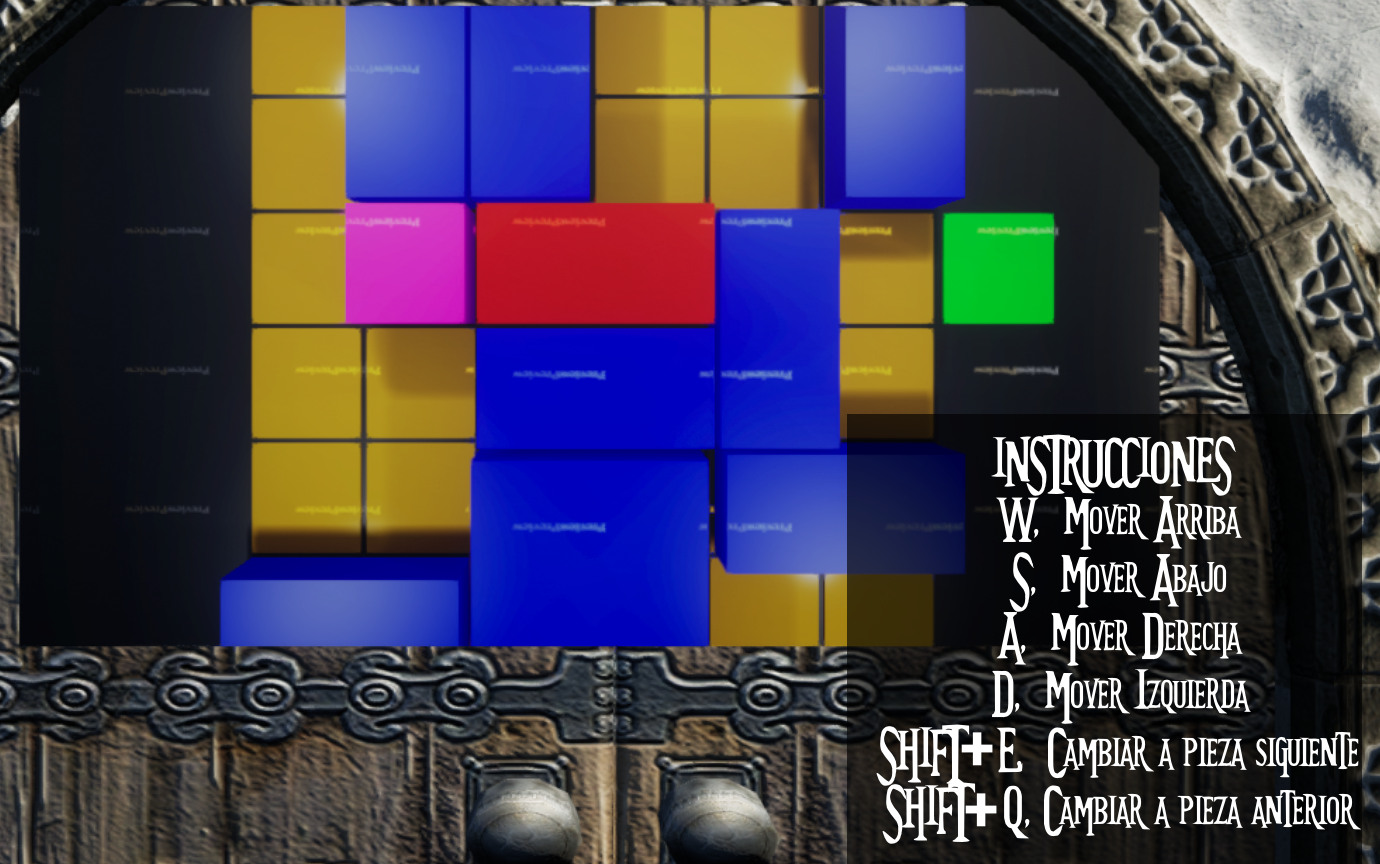
\includegraphics[width=12cm]{./images/Minijuego.png}
  \caption{Ejecución del minijuego durante una partida de \textit{Alliance}}
  \label{Minijuego}
\end{figure}

Durante la ejecución del minijuego, el jugador que lo está jugando no puede moverse ni atacar.


\subsection{¿Cómo incrementar la vida y la estamina?}

La vida y la estamina son los dos rasgos más importantes que posee el jugador. La vida es necesaria para no perder la partida y la estamina es necesaria para poder realizar ataques y para poder correr más rápido. Por esto, se han implementado dos métodos para poder aumentar dichas cualidades.

\begin{itemize}
\item Tanto la vida, como la estamina, se regeneran con el tiempo. Este porcentaje de regeneración es muy bajo, aunque en situaciones de calma en las que no haya combate es muy útil para comenzar los siguientes combates bien regenerado.

\item Existen cajas, barriles y otros destructibles (véase la Figura \todo{Añadir figura de destructibles}). Al romper estos objetos, existe la posibilidad de que aparezcan \textit{pickups} (véase la Figura \todo{Añadir figura de pickups}), que al cogerlos proporcionan vida y estamina.

Coger un \textit{pickup} de vida te aumenta en \todo{Poner cuánto aumenta la salud} puntos tu salud, mientras que coger un \textit{pickup} de estamina aumenta en \todo{poner cuanto aumenta la estamina} puntos tu estamina.
\end{itemize}


\subsection{¿Cómo cambiar el personaje del juego?}

Mientras se está jugando no existe la posibilidad de cambiar el personaje que es controlado por el jugador y continuar con el juego. Existen dos formas de cambiar el personaje, pero ambas necesitan empezar el juego de nuevo:

\begin{itemize}
\item Dejar que los enemigos nos maten. En la pantalla que sale cuando el jugador pierde (se puede ver en la Figura \todo{Insertar imagen cuando el jugador pierde}), hacer click en <<Volver al Menú>>. Una vez en el menú, se puede iniciar una nueva partida escogiendo al personaje que se quiera, entre los dos disponibles.
\item Pausar el juego, presionando la tecla \texttt{P} y hacer click en <<Salir del juego>>. Reiniciar \textit{Alliance} e iniciar una nueva partida, escogiendo al personaje deseado entre los dos personajes disponibles.
\end{itemize}

\renewcommand\bcStyleTitre[1]{\large\hspace*{1.8in}\textcolor{red!100}{#1}}
\begin{bclogo}[
  couleur=red!15,
  arrondi=0.25,
  logo=\hspace*{1in}\bctakecare,
  barre=none,
  noborder=true]{\hspace*{0.15in} Advertencia.}
\itshape \vspace*{0.15in}
\textit{Alliance} no implementa un sistema de guardado de partidas, por lo que si sales de una partida para cambiar tu personaje y empezar una partida nueva, no se guardará tu progreso y tendrás que empezar desde el principio.
\end{bclogo}


\subsection{¿Cómo ver los créditos de \textit{Alliance}?}
\begin{itemize}
\item En primer lugar, haz click en el ejecutable de \textit{Alliance}, para iniciar la aplicación.
\item Aparecerá el menú principal del juego, que se puede ver en la figura \ref{MenuPpal}.
\item En este menú haremos click en <<Creditos>> para visualizar los créditos del videojuego.

\begin{figure}[H]
  \centering
  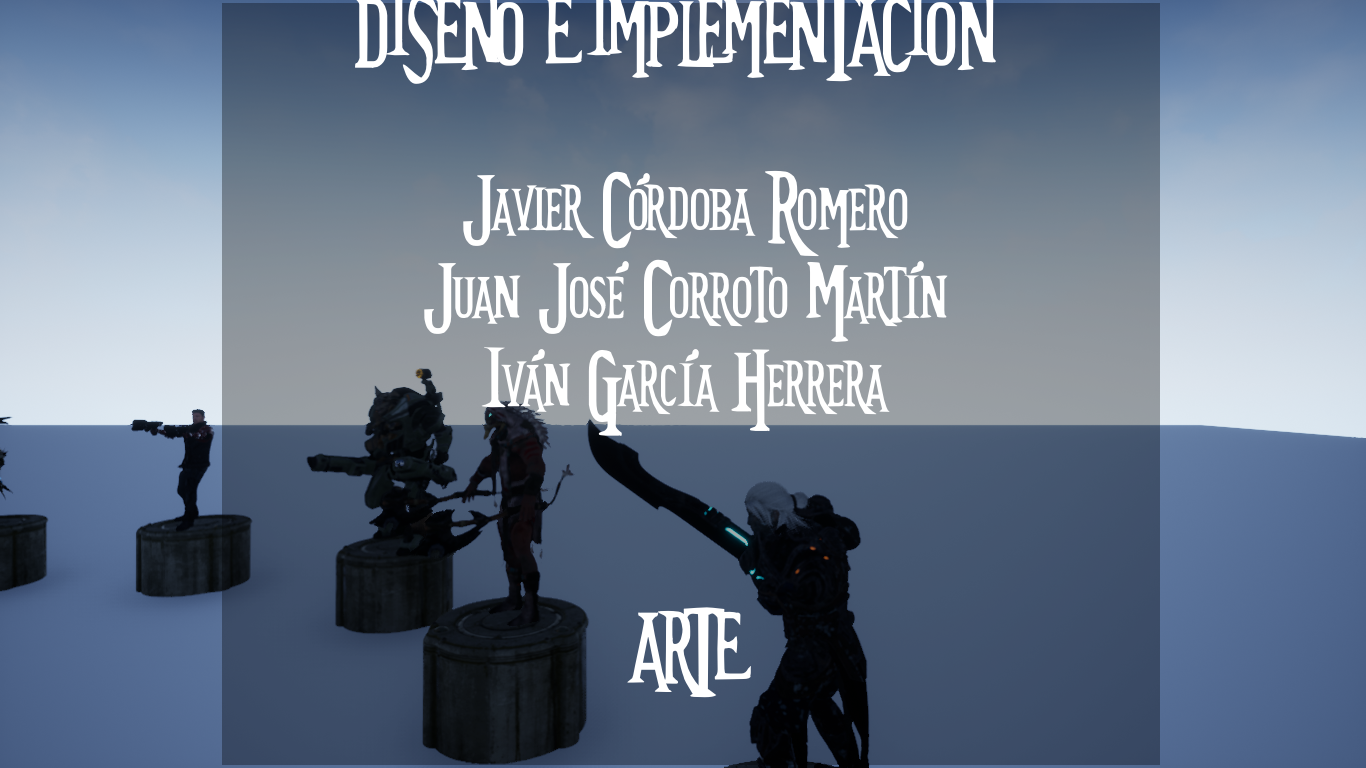
\includegraphics[width=12cm]{./images/Creditos.png}
  \caption{Créditos del juego}
  \label{Creditos}
\end{figure}

\item Se mostrará una interfaz como la de la figura \ref{Creditos}, en la cual se mostrarán los créditos de \textit{Alliance} con una animación de abajo a arriba. Cuando se hallan mostrado todos los créditos, se activará la opción de volver al menú principal del juego.
\end{itemize}
